
% Many thanks to Andrew West for writing most of this file
% Main LaTeX file for CIS400/401 Project Proposal Specification
%
% Once built and in PDF form this document outlines the format of a
% project proposal. However, in raw (.tex) form, we also try to
% comment on some basic LaTeX technique. This is not intended to be a
% LaTeX tutorial, instead just (1) a use-case thereof, and (2) a
% template for your own writing.

% Ordinarily we'd begin by specifying some broad document properties
% like font-size, page-size, margins, etc. -- We have done this (and
% much more) for you by creating a 'style file', which the
% 'documentclass' command references.
\documentclass{sig-alternate}

% These 'usepackage' commands are a way of importing additional LaTeX
% styles and formattings that aren't part of the 'standard library'
\usepackage{mdwlist}
\usepackage{url}
\usepackage{listings}

\begin{document}
\pagenumbering{arabic}

% We setup the parameters to our title header before 'making' it. Note
% that your proposals should have actual titles, not the generic one
% we have here.
\title{CodeScore Progress Report}
\subtitle{Dept. of CIS - Senior Design 2013-2014\thanks{Advisor: Chris Murphy (cdmurphy@cis.upenn.edu).}}
\numberofauthors{4}

\author{
	Allison Pearce \\ \email{alpearce@upenn.edu} \\ Univ. of Penn \\ Philadelphia, PA
	\and Spencer Lee \\ \email{lesp@upenn.edu} \\ Univ. of Penn \\ Philadelphia, PA
	\and Tanvir Ahmed \\ \email{tanvir@upenn.edu} \\ Univ. of Penn \\ Philadelphia, PA
\and Will McDermid \\ \email{wmcd@upenn.edu} \\ Univ. of Penn \\ Philadelphia, PA}

\date{}
\maketitle

% Next we write out our abstract -- generally a two paragraph maximum,
% executive summary of the motivation and contributions of the work.
\begin{abstract}
	\textit{The technology industry lacks automated tools for evaluating software
		quality. These tools would be helpful for individuals desiring to improve
		their abilities, recruiters searching for top programmers, and educators
		needing to quickly assess student performance. We are in the process of
		developing an application called CodeScore that assesses internal software
	quality by detecting code smells. Code smells are easily recognized design
weaknesses that may indicate more significant problems within the system. The
program will recognize code smells using a set of specific rules. It will then
use the results to compute a CodeScore: a single value that reflects the
maintainability and understandability of the piece of software based on the
presence of code smells. }
\end{abstract}

% Then we proceed into the body of the report itself. The effect of
% the 'section' command is obvious, but also notice 'label'. Its good
% practice to label every (sub)-section, graph, equation etc. -- this
% gives us a way to dynamically reference it later in the text via the
% 'ref' command.
\section{Introduction}
\label{sec:intro}
Software failures result in annoyed users at best, and they can cause
catastrophic system failures at worst. Six people received massive radiation
overdoses from a radiation therapy device in one of the canonical examples of a
fatal software error \cite{leveson1995therac}. Failures are consequences of poor
software quality. Software quality is defined as ``conformance to explicitly
stated functional and performance requirements, explicitly documented
development standards, and implicit characteristics that are expected of all
professionally developed software" \cite{pressman1997}. In addition to causing
failures, disregard for software quality is expensive and inefficient, requiring
more dollars and man-hours to maintain, test, and add features to a project than
should be necessary. An increasing appreciation of well-designed software has
been manifested in the international standard for software quality, ISO/IEC
25010. The standard affirms the importance of specifying and measuring
characteristics of quality, and it defines quality models intended to aid in
accomplishing these goals \cite{iso2011iec}.

Software quality is commonly divided into internal quality and external quality.
External quality describes how well the software meets performance expectations,
and encompasses characteristics such as correctness, accuracy, integrity,
robustness, reliability, usability, adaptability, and efficiency. Internal
quality describes how well the software was designed and implemented, and is
concerned with maintainability, flexibility, portability, reusability,
readability, understandability, and testability
\cite{mcconnell1993codecomplete}. Internal and external quality are closely
related, and deficiencies in internal quality lead to deficiencies in external
quality. For example, code that is difficult to understand will also be
difficult to adapt to new requirements, and code that cannot be easily tested
will likely be incorrect or unreliable. 

One way to diagnose internal quality issues is by detecting code smells. Code
smells are easily recognized design weaknesses on the surface of the code that
may indicate deeper, more significant problems within the system. Some common
code smells include:
\begin{itemize}
	\item Classes or methods that have too many lines of code
	\item Duplicated code
	\item Long lists of parameters for functions
	\item Overly complex conditional logic
	\item Inconsistent or uncommunicative naming conventions
	\item Feature envy, a problem in which methods in one class repeatedly use
		data and methods from another class
\end{itemize}

Individual code smells are directly related to problems with specific aspects of
internal quality. For example, overly complex conditional logic and inconsistent
naming conventions detract from understandability and readability. Duplicated
code implies that changes will have to be made not once but everywhere that the
duplication occurs, which detracts from maintainability. 

CodeScore tests for the presence of code smells in order to evaluate internal
quality. We have defined rules for custom algorithms to detect code smells, and
the results of the detection are used compute an internal quality score for a
code sample. The program focuses specifically on how code smells relate to two
elements of internal software quality, maintainability and understandability.
These elements are underemphasized in most classroom settings. Students work
quickly and haphazardly to meet deadlines and never revisit their program after
turning it in, so there is no need to write maintainable or understandable code.
However, understandability and maintainability are critical outside of the
classroom, where teams of developers need to understand code they did not write,
and to maintain it for years as the product evolves. CodeScore will help
students assess and improve these necessary software engineering skills by
providing objective feedback to make them aware of their weaknesses. Computer
science teachers can use the the application when grading assignments to assess
quality without spending hours reading through each student's source code. It
will also allow recruiters to identify potential employees who will contribute
to their company's products with a high regard for quality. Overall, this tool
will help the technology industry to train and recruit a strong developer
workforce who will write programs that are internally sound. 

\section{Related Work}
\label{sec:related_work}
Before describing our methods, we will provide background information
on the different methods of analyzing code, the standards for measuring code
quality, and various services and applications that already strive to provide
quantitative analyses of code quality.


\subsection{Code Analysis Methodologies}
The majority of existing applications for measuring code quality rely on
well-established code analysis techniques. These techniques involve breaking
code down into specific units for processing. Such
techniques include parsing the source code into control structures
\cite{mccabe1976complexity}, tokens \cite{halstead1977elements}, assembly
instructions \cite{park1992software}, or objects \cite{chidamber1994metrics}.
Once the source code has been parsed into some unit (this process is called
static analysis), the attributes of the code, such as reliability, security,
efficiency, size, and maintainability can be measured by calculating various
metrics using the parsed results.
The actual approach to measuring these attributes originated in
\cite{boehm1976quantitative} and later became part of the ISO/IEC 25000 series
of standards relating to the quality and evaluation of software
\cite{iso2011iec}. These techniques and standards comprise the foundation for
today's code quality measurement applications, and they are the basis for our
approach, as well.

\subsection{Ohloh}
Launched in January of 2006, Ohloh \cite{allen2009ohloh} is web service and
online community owned by Black Duck Software which provides basic metrics for
over 650,000 open source projects containing over 24,000,000,000 lines of code
located in over 620,000 source code repositories and managed by more than
3,000,000 contributors. These projects are retrieved from source control
repositories and analyzed. Metrics such as lines of code, amount of source code
comments, and estimated software cost (based on the COCOMO model
\cite{boehm2000software}) are provided, along with commit statistics, project
activity, and programming language detection. This data is graphically displayed
when one views a project's information on the site. Ohloh also provides global
statistics across all projects for different programming languages and
contributor statistics for different authors of open source code. 

Ohloh primarily focuses on tracking project/contributor activity for large
open-source projects. CodeScore focuses more on providing code quality-oriented
metrics.

\subsection{Common Weakness Enumeration}
The Common Weakness Enumeration (CWE) \cite{mitre2006cwe} is a
community-developed list of software weaknesses hosted by the MITRE Corporation.
The CWE was developed with the intention of providing:

\begin{itemize}
	\item a common standard of identifying, mitigating, and preventing software weaknesses.
	\item a common source of measuring weaknesses for software security tools.
	\item a common language for describing the various types of software
		weaknesses that exist in computer architecture, software design, and
		source code.
\end{itemize}

CWE supports the discovery of common types of software security flaws such as
buffer overflows, handler errors, pathname traversals, and resource management
errors (amongst others) within code.

%CWE began with the Common Vulnerabilities and Exposures (CVE) list in 1999 \cite{mitre2005cve}. As part of the SAMATE project \cite{nist2005samate}, MITRE later expanded upon the CVE list with the Preliminary List of Vulnerability Examples for Researchers (PLOVER) \cite{christey2005plover}. PLOVER was the first attempt to take real-world examples of software vulnerabilities and abstract them into common classes of more general vulnerabilities that can arise during the software development process. The goal of PLOVER was to make this information available to developers, researchers, and analysts so that they may use it for a variety of purposes, with the goal of improving code security. CWE encompasses much of the CVE list and expands upon PLOVER by establishing community-developed definitions and descriptions of these common weaknesses.

The Preliminary List of Vulnerability Examples for Researchers (PLOVER)
\cite{christey2005plover} was an early form of CWE. PLOVER was the first attempt
to take real-world examples of software vulnerabilities and abstract them into
common classes of more general vulnerabilities that can arise during the
software development process. The goal of PLOVER was to make this information
available to developers, researchers, and analysts so that they may use it with
the goal of improving code security. CWE expands upon PLOVER by establishing
community-developed definitions and descriptions of these common weaknesses.

CWE primarily strives to provide standards relating to the weaknesses of code in
terms of security. This may be a valuable resource as we develop additional features for
CodeScore, as many security weaknesses are indicative of, or are themselves, code 
smells, but our project has a wider scope. CWE also incorporates community feedback in
developing definitions of weaknesses, which is a strategy we also intend to use
in verifying and fine-tuning our models.

\subsection{HIST}
Historical Information for Smell deTection, or HIST \cite{palomba}, is an
approach developed to detect five specific code smells using change history from
version control systems.  The developers of HIST point out that not all code
smells are possible to detect using just source code because some are by
definition characterized by how the code changes during the project's
development. One example is parallel inheritance hierarchies, in which ``every
tme you make a subclass of one class, you have to make a subclass of another"
\cite{fowler1999}. Though revision histories often display changes at a
file-level granularity, they use a tool called the Change History Extractor to parse
changes at a method- and class-level granularity, and then they identify code 
smells from the parsed logs using specific rules. CodeScore will soon
make use of a similar strategy for incorporating version control information
into several metrics, but CodeScore's analysis includes many more metrics than just
those that can be detected using revision logs.

\begin{figure*}[ht]
	\begin{center}
		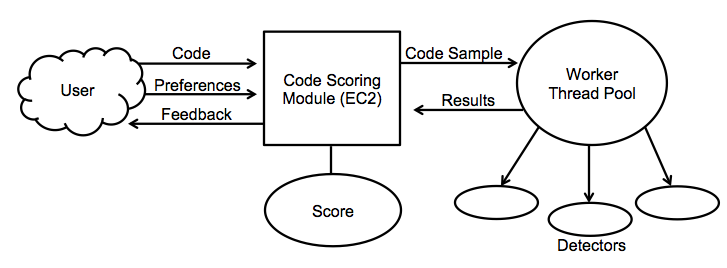
\includegraphics[width=0.9\linewidth]{block_diagram}
	\end{center}
	\vspace{-12pt}
	\caption{System architecture}
	\label{fig:some_graph}
\end{figure*}

\subsection{JOCS}
Judgment of Code Style (JOCS) was a CIS 400/401 project in the 2012-2013
academic year [CITE THIS SHIT]. Their goal was to create a tool for an automated
analysis of code style. Such a tool would be useful is assigning the style grade
often associated with assignments in introductory programming classes, such as
CIS 110 or 120 at the University of Pennsylvania. Features of interest included
line length, modularity, and consistency. They used machine learning to compute
a single score from the features. CodeScore will make use of similar techniques,
but the two projects will be using mostly non-overlapping feature sets and
different strategies for identifying them. Our focus is not on style but on code
smells as they relate to internal quality, which ultimately affects the
correctness, efficiency, and overall external quality of the program. 

\subsection{Other Static Code Analysis Tools}
A wide variety of other static code analysis tools also exist. The Web Application Security Consortium provides a community-sourced list of some commonly used tools for code analysis \cite{webappsec2012}. Some of these tools include:

\begin{itemize}
	\item CodeSonar - A full-featured code analysis tool with binary analysis, results visualization, and a wide variety of metrics. CodeSonar can detect numerous code faults and security risk within projects containing up to millions of lines of Java, C, or C++ code \cite{grammatech2013codesonar}.
	\item Klocwork Insight - Provides a wide range of metrics related to security and reliability with detailed reports and offers integration with a variety of IDEs \cite{klocwork2013insight}.
	\item FindBugs - An open-source code analysis tool which is capable of detecting many different types of bugs, such as null pointer dereferences or infinite loops, in Java code \cite{pugh2013findbugs}.
	\item Yasca - Another open-source code analysis tool combining the functionality of several similar tools in order to provide quality and security metrics for code written in a wide range of languages \cite{scovetta2007yasca}.
\end{itemize}

\section{System Model}
\label{sec:system_model}


CodeScore offers a novel solution amongst all of these existing tools.
Most of the current applications are principally concerned with security,
reliability, correct functionality, efficiency, and other aspects of external quality. Our tool 
focuses on internal quality, which can help prevent problems with external
quality, thus allowing developers to spend less time testing and fixing bugs and
more time on new products and features. Additinally, many of the existing tools
target industry developers, but one of our primary target audiences will be
students, who need to need to develop an appreciation for internal quality
before entering the workforce or academia. Finally, our solution attempts to
provide more functionality than the majority of open-source, similar
applications. We aim to provide quality of functionality similar to
commercial-grade applications, while making our solution accessible to a wider
audience and not merely for large companies. 

We have designed a program called CodeScore that quantitatively assesses code
quality. It is an objective tool for performing a task that seems inherently
subjective. However, the characterization of software quality has been the topic
of much discussion in both academia in industry. Using as a foundation the
components of internal quality described in \cite{iso2011iec} and similar
reports, our program further dissects these components into specific patterns
that can be identified in source code. The holistic scoring system is built up
from a large collection of these specific, detectable indicators to provide one
comprehensive measure of quality.

CodeScore focuses on evaluating internal quality and makes use of static code
analyses. This allows for assessment of source code without bias from different
system architectures or environments. Code smells provide a powerful but simple
indicator of internal quality because they are specific and detectable, they
have a clear relationship with internal quality, and because there is
existing work to use as a reference \cite{moha2009duchien}, \cite{palomba}. The
program currently focuses on just two important metrics of internal quality,
understandability and maintainability. 

\emph{Understandability} is a measure of how easy a code sample is for a human to
interpret. It can be estimated in part by the length of message chains (a code
smell in which one method invokes another, which invokes another, and so on in a
long one-line sequence of function calls), length of parameter lists, by
determining what fraction of variable names are dictionary words versus strings
of letters and numbers, and by analyzing the class structure of a program. 

\emph{Maintainability} is a measure of how easy a code sample will be to update
and change. It can be estimated in part by detecting and recognizing coupling
between classes, duplicated code, and classes that are too large. Another
indicative code smell is shotgun surgery, which describes the situation in which
changing one behavior requires numerous changes to code in different places. For
example, if logging statements are implemented separately in each function in a
class, then adding line numbers to the logs will require considerable time and effort. A
better solution would be to write a log wrapper for all of the functions, so
that any changes only need to be made once. 

CodeScore implements the workflow illustrated in Figure \ref{fig:some_graph}. The
key components of the system are the main driver and thread pool, the detectors,
and the scoring module. First, a user uploads source code, an optional
revision history from a version control repository, and a JSON file of
preferences to our server. Detectors for several code smells related to
understandability and maintainability run in parallel on all files in the source
code and the revision history. The results of the detections are then combined 
into an overall score for the code sample, analogous to a grade on an essay. The program 
also provides a detailed score report describing the number, type, and location of
problems in the code. This report can be shared with recruiters as a quick and objective
evaluation of a candidate's programming ability, used as a tool for
self-improvement, or incorporated into teachers' grading rubrics. 

The detectors are the most complicated component of the system and present the
most technical challenges. Each code smell requires a unique detection
algorithm, sometimes involving analysis of multiple classes together or complex
parsing. The detectors currently implemented have been made successful by first
creating a detailed list of all possible patterns to search for using the
syntactical structure of the program, then implementing the search pattern and
a counter to keep track of the number of violations. For any detectors that
require some sort of threshold, like the maximum depth allowed for nested
conditionals, the program's default parameters can be overriden using a
preference configuration file.

Some code smells cannot easily be detected using the source code, but
can be found by taking advantage of additional information. For instance, assume
every time a method A.foo() is changed, several additional changes must be made
elsewhere in the code. This issue would be evident upon careful inspection of the
revision history but difficult to detect in the source code itself. This is one
of the next features that we plan to incorporate into CodeScore. The challenging
implementation is discussed in the next section. Adding revision history analyses
to our list of metrics will help CodeScore offer a more well-rounded assessment of software
projects, and they are high priorities among our next steps.

Another challenge is making the program efficient. CodeScore is designed to run
on large and small software projects, which means that all parsing, processing,
and reporting must be carefully engineered to produce results in a timely
manner. CodeScore employs parallel processing techniques so that the runtime
scales well with the number of metrics and the size of the input, and it takes
advantage of efficient parsing APIs to assist with code smell detection.


\section{System Implementation}
\label{subsec:approach}

All processing for CodeScore happens on an Amazon EC2 cloud processing machine.
EC2 is a service that provides resizable computing capacity in the cloud. 
Users upload Java code, a preferences file, and an optional revision
history from a version control repository to the EC2 instance through a simple web app. The preferences 
file is encoded in JSON and includes information that is specific to each detector, 
such as thresholds for certain code smells. A sample preferences file can be
seen in Figure \ref{fig: json}. If no preferences
file is includes, the program uses default values. The controller class and all
detectors are implemented in Java. 
When software is uploaded to the endpoint, the controller class
generates $n$ worker threads, where $n$ is the number of detection algorithms to be
performed on the software sample. Currently, $n=3$ since we support $3$
detectors, but we hope to eventually implement 8 to 12 detectors. 
Each of the workers performs a specific detection task on the uploaded files.
Once complete, the controller then reduces all of the data computed by the workers and
summarizes the findings. A maintainability score and an understandability score
are computed using the results of the relevant code smell detection
algorithms. The scores are informed by the frequency and severity of the
issues (one poorly named variable is less problematic than five duplicated code
blocks), and the sum of these two scores is reported as the overall
CodeScore. The scoring algorithm has not been fully implemented, but it will
assign a weight the results from each of the code smell detectors based on how
strongly each code smell impacts internal code quality. As a starting point,
these weights can be configured with the user preferences file. Later, these
weights will be tuned using feedback from user studies, in which other people
will be asked to rate the severity of various code smells with regard to their
affect on internal software quality.

\begin{figure}[ht]
	\begin{center}
		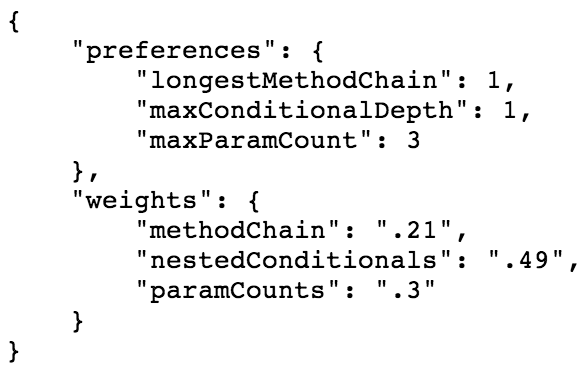
\includegraphics[width=0.9\linewidth]{json}
	\end{center}
	\vspace{-12pt}
	\caption{User preferences file encoded in JSON}
	\label{fig: json}
\end{figure}


The detectors use the Eclipse Java Abstract Syntax Tree (AST) API to parse the Java code
as a first step in finding code smells. Traversing the AST allows the system to access and manipulate Java code
at the syntactic level, efficiently searching for specific elements such as if
statements or method declarations. Detecting code smells at the AST level will
also make CodeScore easy to adapt to additional programming languages in the future.
Most object-oriented code smells have the same properties from the perspective of the AST,
which abstracts away the specifics of individual programming languages. 

A sample abstract syntax tree and the Java code it represents can be seen in Figure~\ref{fig: ast}.

\begin{figure*}[ht]
	\begin{center}
		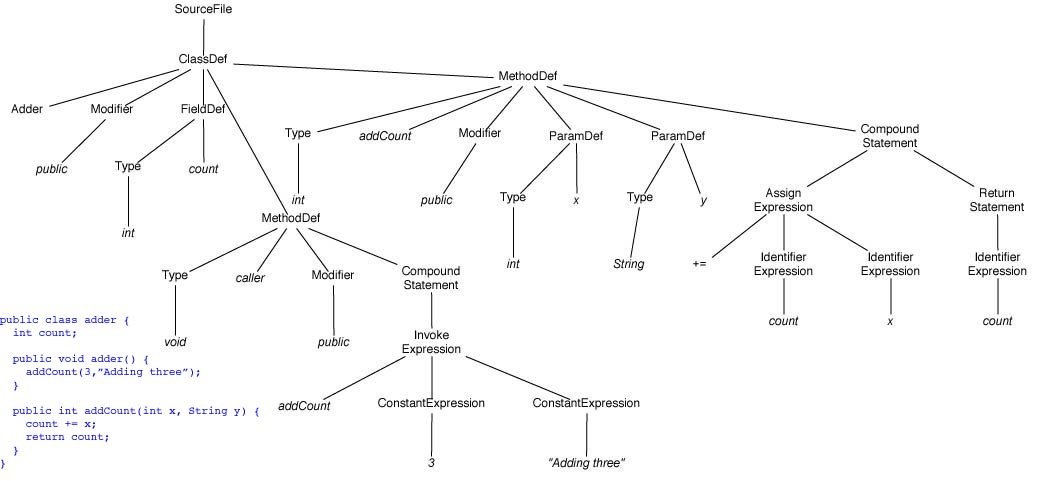
\includegraphics[width=0.9\linewidth]{syntax_tree}
	\end{center}
	\vspace{-12pt}
	\caption{Sample Java abstract syntax tree}
	\label{fig: ast}
\end{figure*}

We have prioritized the code smells and have implemented three of them so far.
Some code smells are simpler to detect than others, and we currently have
detectors for the following:

\begin{itemize}
	\item Long parameter lists. Method declarations are parsed using the AST
		API, and then parameter lists are extracted to determine their length.
		The maximum length parameter list can be configured from the JSON
		preferences file.
	\item Deeply nested conditional logic. Conditional statements including if
		statements and loops are parsed using the AST API. Traversing the
		program as a tree results in finding parent-child relationships between
		nested conditional statements. The maximum nesting depth is configurable
		from the preferences file. 
	\item Message chaining. Method invocations can be isolated using the AST
		API. By examining the context information provided by the AST API about
		each method invocation, it is possible to detect when multiple method
		calls are chained together. The maximum length of chaining to allow is
		configurable in the preferences file.
\end{itemize}

All of these code smells detract from understandability. Poor naming conventions
also detract from understandability. We have implemented a basic natural
language processing module using the Apache OpenNLP library. This library will
be used to analyze variable and method names to determine if they are
informative (containing some form of a dictionary word or words) and consistent.
Variable and method declarations can be extracted from the source code using the
AST API. 

Code smells that affect both understandability and maintainability are long methods
and large/complex classes. Both of these will be detected by finding the class
or method declaration using the AST and analyzing the contents for length.
Additionally, to measure class complexity, measures such as the McCabe
Cyclomatic Complexity [**CITE THIS**] can be calculated. 

Code smells that affect primarily maintainability are duplicated code,
feature envy, and shotgun surgery. The Java Reflection API [**CITE THIS TOO**]
faciliates duplicate code detection. Feature envy, indicative of an
inappropriate relatinship between two classes, will require a more in-depth
analysis several structures in the AST. We can find references to each class
field and method invocation within a particular class and determine if they
correspond to a different class or the class being examined. 

Shotgun surgery is a code smell affecting maintainability that requires more
than just the source code to detect. As described previously, shotgun surgery is
a problem in which changing one behavior requires several separate changes in
the code.  This antipattern can be detected by parsing revision histories to
determine if certain methods or lines of code in different parts of the program
tend to changed at the same time. Analyzing revision history will require the development 
of a custom parser that can extract and tokenize changes at a method-level
granularity. We can do this by extracting a full change history (such as a git
diff of two consecutive commits), removing the metadata symbols (for example, git uses plus
symbols and minus symbols to indicate insertions and deletions) to extract just
the code, and then using the Java AST API to examine the syntactic structure of
the elements that were changed. The shotgun surgery detector will analyze the
full history of the program, keeping track of which methods are modified
together in order to see if a problematic pattern exists.

One drawback of the overall CodeScore system is that it is largely centralized.
If the server containing the controller code is compromised at any time during
the computation, all progress in the analysis will be lost. A reach goal or
future development is to decentralize the process so that loss of a server does
not result in complete loss of progress. Ideally, this could be implemented
using MapReduce \cite{dean2008mapreduce}.

\section{System Performance}
At this stage in the implementation of CodeScore, there are two key aspects of
our application that can be tested:

\begin{itemize}
	\item How accurately code smells are detected.
	\item How quickly the analysis runs.
\end{itemize}

The detectors have been tested primarily with smaller code samples which were purposely
polluted with the code smells we were seeking to detect: long parameter lists,
deeply nested conditional logic, and message chaining. These code samples were
analyzed by hand to construct an oracle from which we could judge the system's performance.

The system detected $100\%$ of the code smells that were found by hand, which
corresponds to $100\%$ precision and recall. It should be noted that CodeScore
is currently only equipped with three of the simpler code smell detectors, and we
expect these scores to be lower, perhaps $80\%$ after incorporating more complex
detection algorithms.

The speed of execution varied roughly linearly with the number of lines of code in
preliminary tests. The bottleneck in runtime appears to be the Java Abstract
Syntax Tree API. At this time, the benefits of using the AST API in terms of simplicity and
modularity outweigh any added slowness in processing. However, we will
investigate alternative methods if runtime with future detection algorithms
becomes a serious issue. See Figure~\ref{fig:runtime} for a graph of the runtime analysis results.

\begin{figure}
	\begin{center}
		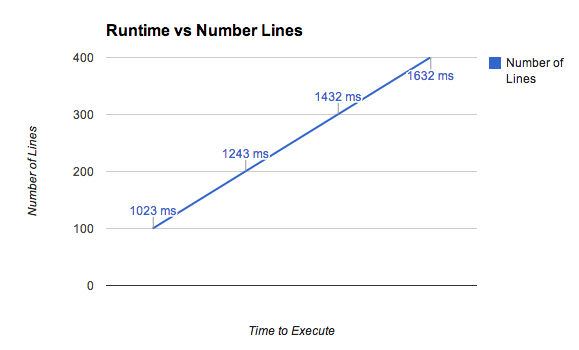
\includegraphics[width=0.9\linewidth]{CodeScoreRuntimeGraph}
	\end{center}
	\vspace{-12pt}
	\caption{Preliminary Runtime Analysis of CodeScore Module}
	\label{fig:runtime}
\end{figure}

\section {Remaining Work}
We have a basic end-to-end system in place, so our focus now is to add features and expand our set of code smell detectors. The remaining steps are:
\label{sec:research_timeline}
\begin{itemize*}
	\item Implement  minimum of five more detection algorithms, including:
		\begin{itemize*}
			\item Duplicated code
			\item Poor naming conventions
			\item Feature envy 
			\item Shotgun surgery
			\item Complex classes
		\end{itemize*}
	\item Create a scoring algorithm that computes a single score based on the findings of the detectors. Allow this scoring algorithm to be configured by a JSON file. 
	\item Move the code so that it runs on EC2 instead of running locally. Create web front-end for users to upload their code.
	\item Perform user studies to compare CodeScore's grade to human evaluation. Incorporate feedback to improve detection and scoring algorithms.
\end{itemize*}
Additionally, if the previous goals are accomplished earlier than expected, we will investigate how to change design to use map reduce. We will also look for more code quality metrics to incorporate and add additional code smells. 

It is possible that once we have implemented all of the detectors, not all of
the code smells will provide unique information. Some code smells might be so correlated with each other that
performing the additional detection is not worth the increased processing time.
If this is the case, we will discard one of the correlated smells and replace it
with a more informative metric.

We estimate that we have completed 40\% of the necessary tasks for CodeScore.


% We next move onto the bibliography.
\bibliographystyle{plain} % Please do not change the bib-style
\bibliography{main}  % Just the *.BIB filename

% Here is a dirty hack. We insert so much vertical space that the
% appendices, which want to begin in the left colunm underneath
% "references", are pushed over to the right-hand column. If we looked
% hard enough, there is probably a command to do exactly this (and
% wouldn't need tweaked after edits).
\vspace{175pt}

% We then use appendices to share some additional information with
% you, though you won't need appendices in your own proposal.

% The usage of 'enumerate' (similar to 'itemize') we talked about
% above

% You may also notice we have many 'vspace' commands lying
% around. These create 'vertical space' and are a way to force LaTeX
% to cooperate, sometimes. Don't get too involved with using them
% initially, though, because adding or deleting a single line of task
% can dramatically change how LaTeX chooses to format, page, and space
% the document
\end{document} 

